\documentclass[10pt]{article}
\usepackage[margin=3cm]{geometry}
\usepackage{amssymb}
\usepackage{verbatim}
\usepackage{graphicx}
\usepackage{amsmath}
\usepackage{capt-of}
\title{\bfseries\Huge Bram van den Akker}

\date{}
\begin{document}
\title{Wave equation simulation}
\author{Abe Wiersma, Bram van den Akker}
\date{\today}
\maketitle
\newpage

\section{Openmp vs pthreads}
Figure 1 shows the speeds of 1 to 8 cores using pthreads en openmp with the static, dynamic and guided scheduling at a chunk size of 1000. The effect of multi threading is almost the exactly the same in all different methods. 
Static scheduling has the worst performances of the openmp scheduling methods. This is because the static method does not attempt to find the optimal schedule. When processes are not finishing at the same speed the dynamic and guided scheduling methods can gain performances by allocating the chunks more efficiency.
Our pthreads method has the highest performance. This is because the division of tasks is optimized for the specific task, something openmp is not able to do because of the limited knowledge of specific goal of the program.

\subsection{The effect of chunks sizes}
The three scheduling methods give completely different results with different chunk sizes. 
In figure 2 you can see the effect of chunk sizes in dynamic scheduling. When using a small chunk size the performances is really bad. This is because of the high amounts of overhead the scheduling of small chunks gives. With larger chunks the performances improves extremely due to the loss of overhead to scheduling the high amounts of chunks.

Figure 3 shows the effects of chunk sizes on static scheduling. here you can see that increasing the chunk size improves performance just like in dynamic scheduling although not in such an extreme matter. With larger chunk sizes the overhead of switching and managing chunks will decreased, resulting in better performance.
 
Figure 4 is actually pretty useless, the effect of the chunk size in guided scheduling is not relevant. The chunk size decreases each dispatch and the set chunk size will be ignored. 

\begin{figure}
  \centering
    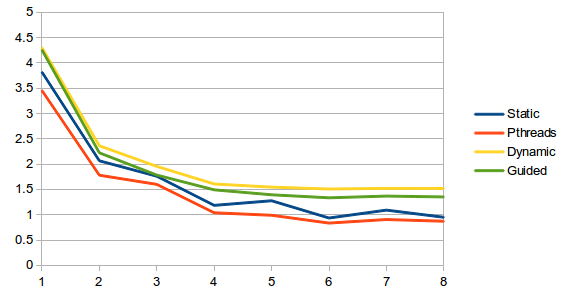
\includegraphics[width=\textwidth]{compare.png}
  \caption{1 to 8 cores with openmp vs pthreads}
\end{figure}
\break
\begin{figure}
  \centering
    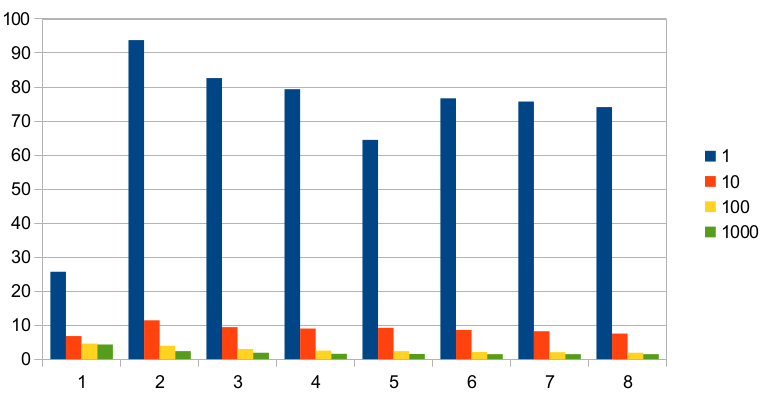
\includegraphics[width=\textwidth]{dynamic.png}
  \caption{1 to 8 cores with openmp and dynamic scheduling.}
\end{figure}
\break
\begin{figure}
  \centering
    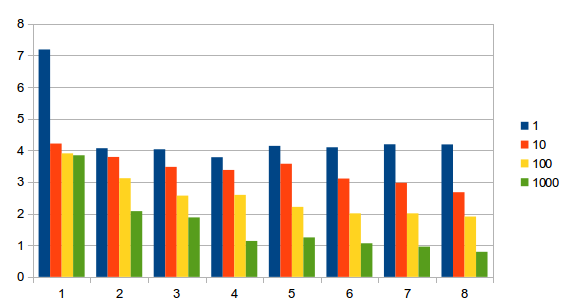
\includegraphics[width=\textwidth]{static.png}
  \caption{1 to 8 cores with openmp and static scheduling.}
\end{figure}
\break
\begin{figure}
  \centering
    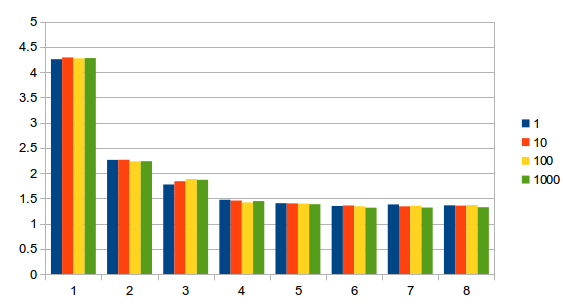
\includegraphics[width=\textwidth]{guided.png}
  \caption{1 to 8 cores with openmp and guided scheduling.}
\end{figure}
\break


\end{document}